\documentclass[11pt,a4paper]{article}

% ---- packages -----
\usepackage[a4paper,margin=2.5cm]{geometry}
\usepackage[onehalfspacing]{setspace}
\usepackage[T1]{fontenc}
\usepackage{lmodern}
\usepackage{microtype}
\usepackage{booktabs}
\usepackage{tabularray}
\UseTblrLibrary{booktabs}
\UseTblrLibrary{siunitx}
\usepackage{float}
\usepackage{graphicx}
\usepackage{amsmath, amssymb}
\usepackage{natbib}
\usepackage[hidelinks]{hyperref}
\usepackage{titlesec}
\usepackage{tikz}
\usetikzlibrary{positioning, arrows.meta}
\titlespacing*{\section}{0pt}{1.0\baselineskip}{0.4\baselineskip}
\titlespacing*{\subsection}{0pt}{0.8\baselineskip}{0.3\baselineskip}

% modelsummary helpers
\providecommand{\tinytableTabularrayUnderline}[1]{\underline{#1}}
\providecommand{\tinytableTabularrayStrikeout}[1]{\sout{#1}}

\title{\textbf{MSS (2004) Revisited:\\
       Weak Instruments and Dynamic Panel Identification}}
\author{Alexander Lievens and Tobias Vanoverschelde\\
\small KU Leuven: D0S91a Advanced Applied Econometrics\\
\small Prof.\ Dr.\ Dirk Czarnitzki}
\date{May 2026}

\begin{document}
\maketitle

% Abstract written last; placeholder for now.
% \begin{abstract}
% \noindent ...
% \end{abstract}

% ===========================================================================
\section{Introduction}\label{sec:intro}
% ===========================================================================
Estimating the causal effect of income shocks on civil conflict is
not an estimation problem but an identification problem. OLS confounds
three biases: conflict destroys output (reverse causation), national
accounts in low-income economies are measured with error, and
persistent country traits affect both (omitted variables). No amount
of data fixes this. The effect is identified only if we can find a
source of variation in growth that is exogenous to conflict and does
not enter the conflict equation directly.

\citet{MSS2004}, henceforth MSS, proposed that source: annual rainfall
growth, used as an excluded instrument for per-capita GDP growth on a
panel of 41 sub-Saharan African countries over 1981--1999. The
identifying assumptions are that rainfall shifts agricultural output
(relevance), and that it affects conflict only through that channel
(exclusion). The paper was novel in 2004. It also predates several of
the diagnostic tools we now use to evaluate IV designs.

The literature that followed targeted each of these assumptions in
turn. \citet{BrucknerCiccone2010} proposed an alternative instrument
based on global commodity prices, relying on a different exogeneity
argument. \citet{Ciccone2011} questioned the specification of the
first stage, showing that rainfall's mean-reversion contaminates the
growth-as-IV interpretation. \citet{Sarsons2015} tested the exclusion
restriction directly, exploiting irrigation infrastructure that breaks
the agricultural channel.

We revisit MSS with two questions. First, how much the original
rainfall design tells us about $\beta$ once modern weak-instrument
diagnostics are applied. Second, whether a dynamic-panel identification
strategy that does not rely on rainfall recovers a coherent estimate.

Section~\ref{sec:identification} formalises the MSS identification.
Section~\ref{sec:critiques} surveys the critiques.
Section~\ref{sec:data} describes the data. Section~\ref{sec:methods}
sets out the estimators. Section~\ref{sec:results} reports estimates.
Section~\ref{sec:discussion} concludes.

% ===========================================================================
\section{The MSS identification strategy}\label{sec:identification}
% ===========================================================================
MSS fit the structural equation
\begin{equation}
C_{it} = \alpha_i + \lambda_i t + \beta\, g^{y}_{it} + \gamma' X_{it} + u_{it},
\label{eq:structural}
\end{equation}
where $C_{it} = \mathbf{1}\{\text{conflict}_{it}\}$ is a binary indicator for civil
conflict in country $i$ at year $t$, $g^{y}_{it} = \Delta \log(\text{GDP}_{it})$ is
per-capita GDP growth, $\alpha_i$ are country fixed effects, $\lambda_i t$ are
country-specific linear time trends, and $X_{it}$ collects time-varying controls
(lagged Polity~2). Opportunity-cost theory \citep{Grossman1991} predicts
$\beta < 0$.

Estimating equation~\eqref{eq:structural} by OLS is inconsistent for the reasons
listed in Section~\ref{sec:intro}. MSS instrument $g^{y}_{it}$ with annual
rainfall growth $g^{R}_{it}$ and its first lag:
\begin{equation}
g^{y}_{it} = a_i + b_i t + \pi_1\, g^{R}_{it} + \pi_2\, g^{R}_{i,t-1}
             + \delta' X_{it} + v_{it}.
\label{eq:firststage}
\end{equation}

The identifying assumptions, made conditional on $\alpha_i$ and $X_{it}$, are:

\textit{Relevance}: $\mathrm{Cov}(g^{R}_{it}, g^{y}_{it}) \neq 0$. Rainfall shifts
agricultural output, which is a large share of African GDP. Testable through the
first-stage $F$ statistic on the excluded instruments.

\textit{Exclusion}: $\mathrm{Cov}(g^{R}_{it}, u_{it}) = 0$. Rainfall affects
conflict only through GDP. Not directly testable in general; with two
instruments, the Sargan test provides one degree of freedom of indirect check on
whether the two rainfall measures imply the same $\beta$.

\begin{figure}[H]
\centering
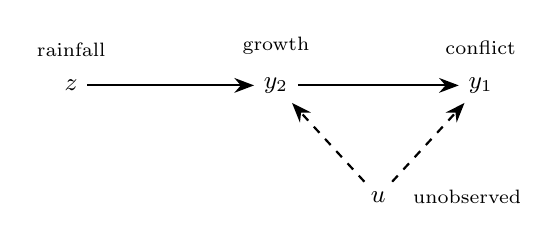
\begin{tikzpicture}[
  node distance=2.6cm,
  every node/.style={font=\small},
  arr/.style={->, >={Stealth[length=2.5mm]}, thick}
]
  \node (z)  {$z$};
  \node[right of=z]  (y2) {$y_2$};
  \node[right of=y2] (y1) {$y_1$};
  \node[below=1.0cm of y2, xshift=1.3cm] (u)  {$u$};

  \draw[arr] (z)  -- (y2);
  \draw[arr] (y2) -- (y1);
  \draw[arr, dashed] (u) -- (y2);
  \draw[arr, dashed] (u) -- (y1);

  \node[above=0.05cm of z]  {\scriptsize rainfall};
  \node[above=0.05cm of y2] {\scriptsize growth};
  \node[above=0.05cm of y1] {\scriptsize conflict};
  \node[right=0.1cm of u]   {\scriptsize unobserved};
\end{tikzpicture}
\caption{The MSS identification strategy as a DAG. Solid arrows show the
assumed causal pathway: rainfall ($z$) affects growth ($y_2$), which affects
conflict ($y_1$). Dashed arrows show unobserved confounders ($u$) that bias
OLS. Identification of $\beta$ requires the $z \to y_2$ arrow (relevance,
testable) and the \emph{absence} of any $z \to y_1$ arrow (exclusion, not
directly testable).}
\label{fig:dag-mss}
\end{figure}

The specification choices matter. MSS use country fixed effects to absorb
time-invariant heterogeneity (geography, institutions, colonial history) and
country-specific linear time trends to absorb slow secular movements
(democratisation, technology diffusion). They do not use year fixed effects,
which would absorb the common component of rainfall shocks across the panel
and reduce the variation the instrument exploits. Standard errors are clustered
at the country level.

Their preferred 2SLS specification yields $\hat\beta \approx -2.4$: a
five-percentage-point decline in growth raises the probability of conflict by
roughly twelve percentage points.

% ===========================================================================
\section{Methodological critiques and alternative identification}\label{sec:critiques}
% ===========================================================================
The literature that followed MSS extended the design along three axes:
it offered alternative instruments, questioned the first-stage
specification, and tested the exclusion restriction directly. Only the
last two are critiques in the strict sense; the first is a parallel
identification strategy.

\textbf{Alternative instrument.} \citet{BrucknerCiccone2010} replace
rainfall with country-specific commodity export price shocks: the
weighted sum of global commodity prices, using each country's export
composition as weights. The exogeneity argument is small-country
price-taking. Global commodity prices are determined on world markets,
and no single sub-Saharan African country is large enough to move them.
Their first stage becomes
\begin{equation}
g^{y}_{it} = a_i + \tilde\pi\, \text{shock}^{P}_{it}
             + \tilde\delta' X_{it} + v_{it},
\label{eq:bc-fs}
\end{equation}
while the structural equation~\eqref{eq:structural} is unchanged. They
recover a negative and significant $\beta$, corroborating the MSS sign
under a different identifying assumption. This is identification
pluralism rather than critique: two unrelated exogeneity arguments
converge on the same conclusion, which strengthens MSS rather than
weakens it. Within MSS's own design, the analogue is the Sargan
over-identification test on the two rainfall instruments
(current and lagged); we return to it in Section~\ref{sec:results}.

\textbf{Specification critique.} \citet{Ciccone2011} attacks the
functional form rather than the exogeneity. Rainfall is mean-reverting:
an unusually wet year tends to be followed by drier years, so rainfall
growth carries a mechanical negative serial correlation with the past
level of rainfall. If conflict responds to rainfall \emph{levels}
(drought leads to a bad harvest, which raises conflict), then
instrumenting growth with rainfall growth captures a level-driven
effect dressed up as a growth effect. He re-runs the analysis with
rainfall levels as the IV and finds the effect attenuates substantially.
\citet{MiguelSatyanath2011} reply defending the original parameterisation.
The lesson is generic: 2SLS consistency requires correct first-stage
specification, not just instrument exogeneity. An exogenous instrument
applied in the wrong functional form still produces an inconsistent
estimate.

\textbf{Direct test of exclusion.} The most consequential critique
tests the exclusion restriction itself. \citet{Sarsons2015} uses Indian
rainfall and conflict data combined with records of irrigation dams.
In regions \emph{downstream of dams}, water supply is decoupled from
local rainfall: the agricultural-income channel is physically broken.
If MSS's exclusion holds (rainfall affects conflict only through
agricultural income), then in dam-downstream regions rainfall should
not predict conflict. She finds that it does. The implication is a
direct $z \to y_1$ arrow that the MSS DAG denies (Figure~\ref{fig:dag-sarsons}).

\begin{figure}[H]
\centering
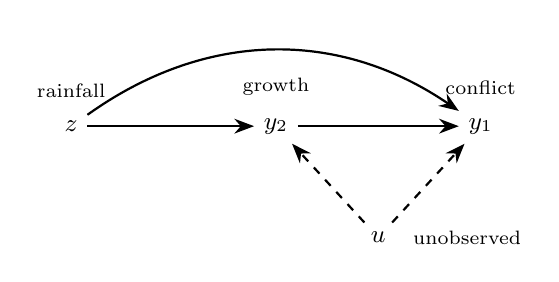
\begin{tikzpicture}[
  node distance=2.6cm,
  every node/.style={font=\small},
  arr/.style={->, >={Stealth[length=2.5mm]}, thick}
]
  \node (z)  {$z$};
  \node[right of=z]  (y2) {$y_2$};
  \node[right of=y2] (y1) {$y_1$};
  \node[below=1.0cm of y2, xshift=1.3cm] (u)  {$u$};

  \draw[arr] (z)  -- (y2);
  \draw[arr] (y2) -- (y1);
  \draw[arr, dashed] (u) -- (y2);
  \draw[arr, dashed] (u) -- (y1);
  \draw[arr, thick] (z) to[bend left=35] (y1);

  \node[above=0.05cm of z]  {\scriptsize rainfall};
  \node[above=0.05cm of y2] {\scriptsize growth};
  \node[above=0.05cm of y1] {\scriptsize conflict};
  \node[right=0.1cm of u]   {\scriptsize unobserved};
\end{tikzpicture}
\caption{Sarsons's critique as a DAG. Same diagram as
Figure~\ref{fig:dag-mss}, plus a direct $z \to y_1$ arrow that exclusion
denies. Evidence from regions where the $z \to y_2$ channel is
physically blocked (downstream of dams) supports the existence of this
arrow.}
\label{fig:dag-sarsons}
\end{figure}

The methodological lesson is general. Exclusion restrictions are
sometimes partially testable: if the IV is claimed to operate through
one channel, find a setting where the channel is shut and check whether
the IV still moves the outcome. The post-2015 standard for IV papers in
development economics has internalised this test.

% ===========================================================================
\section{Data}\label{sec:data}
% ===========================================================================
We use the replication panel distributed by MSS via the Harvard
Dataverse (doi:10.7910/DVN/27324). It covers 41 sub-Saharan African
countries over 1981--1999. After constructing one lag of GDP growth and
dropping country-years with missing controls, the estimation sample is
702 country-year observations.

The outcome \texttt{any\_prio} is a PRIO indicator equal to one if a
country experiences at least 25 battle deaths in a year. The endogenous
regressor \texttt{gdp\_g} is annual per-capita GDP growth. The excluded
instruments are current and lagged rainfall growth, \texttt{GPCP\_g}
and \texttt{GPCP\_g\_l}, constructed from the Global Precipitation
Climatology Project. Controls follow MSS: initial log income, lagged
Polity~2, ethnic and religious fractionalisation, an oil-exporter
dummy, log mountainous terrain, and log lagged population. Only lagged
Polity~2 is time-varying; the rest are absorbed by country fixed
effects in our preferred specifications.

\begin{table}[H]
\centering
\caption{Descriptive statistics, estimation sample ($N = 702$).}
\label{tab:descriptives}
\begin{tabular}{lrrrrr}
\toprule
Variable & $N$ & Mean & SD & Min & Max \\
\midrule
\texttt{any\_prio}  & 702 & 0.269   & 0.444 & 0.000   & 1.000 \\
\texttt{gdp\_g}     & 702 & $-0.006$ & 0.066 & $-0.474$ & 0.319 \\
\texttt{GPCP\_g}    & 702 & 0.015   & 0.210 & $-0.550$ & 1.680 \\
\texttt{y\_0}       & 702 & 1.16    & 0.90  & 0.316   & 4.84  \\
\texttt{polity2l}   & 702 & $-3.55$ & 5.55  & $-10$   & 9     \\
\texttt{ethfrac}    & 702 & 0.655   & 0.237 & 0.036   & 0.925 \\
\texttt{relfrac}    & 702 & 0.487   & 0.185 & 0.000   & 0.783 \\
\texttt{Oil}        & 702 & 0.117   & 0.321 & 0       & 1     \\
\texttt{lmtnest}    & 702 & 1.58    & 1.43  & 0       & 4.42  \\
\texttt{lpopl1}     & 702 & 8.77    & 1.20  & 5.75    & 11.7  \\
\bottomrule
\end{tabular}
\end{table}

Three features of the panel matter for what follows. The unconditional
conflict frequency is 27\%. Average growth is slightly negative
($-0.6\%$ per annum). The panel is democracy-poor on average (mean
Polity~2 of $-3.5$ on a scale of $-10$ to $10$).

% ===========================================================================
\section{Methodology}\label{sec:methods}
% ===========================================================================
% TODO: POLS, FE/RE, 2SLS, LIML/Fuller, AR, dynamic-panel GMM
% each tied to the DAG, with the assumption + diagnostic test it warrants.

% ===========================================================================
\section{Results and diagnostics}\label{sec:results}
% ===========================================================================
% TODO: main results table + diagnostics table + interpretation.

% ===========================================================================
\section{Discussion}\label{sec:discussion}
% ===========================================================================
% TODO: what the design can and cannot identify; the GMM-rescue conclusion.

% ---------------------- bibliography ----------------------
\renewcommand{\refname}{References}
\begin{thebibliography}{99}\small

\bibitem[Anderson and Rubin(1949)]{AndersonRubin1949}
Anderson, T.W., and H.\ Rubin (1949). ``Estimation of the parameters
  of a single equation in a complete system of stochastic equations.''
  \emph{Annals of Mathematical Statistics} 20(1): 46--63.

\bibitem[Arellano and Bond(1991)]{ArellanoBond1991}
Arellano, M., and S.\ Bond (1991). ``Some tests of specification for
  panel data: Monte Carlo evidence and an application to employment
  equations.'' \emph{Review of Economic Studies} 58(2): 277--297.

\bibitem[Blundell and Bond(1998)]{BlundellBond1998}
Blundell, R., and S.\ Bond (1998). ``Initial conditions and moment
  restrictions in dynamic panel data models.''
  \emph{Journal of Econometrics} 87(1): 115--143.

\bibitem[Bound, Jaeger, and Baker(1995)]{BoundJaegerBaker1995}
Bound, J., D.A.\ Jaeger, and R.M.\ Baker (1995). ``Problems with
  instrumental variables estimation when the correlation between the
  instruments and the endogenous explanatory variable is weak.''
  \emph{Journal of the American Statistical Association} 90(430):
  443--450.

\bibitem[Br\"uckner and Ciccone(2010)]{BrucknerCiccone2010}
Br\"uckner, M., and A.\ Ciccone (2010). ``International commodity
  prices, growth and the outbreak of civil war in Sub-Saharan Africa.''
  \emph{Economic Journal} 120(544): 519--534.

\bibitem[Ciccone(2011)]{Ciccone2011}
Ciccone, A.\ (2011). ``Economic shocks and civil conflict: A
  comment.'' \emph{American Economic Journal: Applied Economics}
  3(4): 215--227.

\bibitem[Fuller(1977)]{Fuller1977}
Fuller, W.A.\ (1977). ``Some properties of a modification of the
  limited information estimator.'' \emph{Econometrica} 45(4):
  939--953.

\bibitem[Grossman(1991)]{Grossman1991}
Grossman, H.I.\ (1991). ``A general equilibrium model of
  insurrections.'' \emph{American Economic Review} 81(4): 912--921.

\bibitem[Miguel et al.(2004)]{MSS2004}
Miguel, E., S.\ Satyanath, and E.\ Sergenti (2004). ``Economic
  shocks and civil conflict: An instrumental variables approach.''
  \emph{Journal of Political Economy} 112(4): 725--753.

\bibitem[Miguel and Satyanath(2011)]{MiguelSatyanath2011}
Miguel, E., and S.\ Satyanath (2011). ``Re-examining economic shocks
  and civil conflict.'' \emph{American Economic Journal: Applied
  Economics} 3(4): 228--232.

\bibitem[Nickell(1981)]{Nickell1981}
Nickell, S.\ (1981). ``Biases in dynamic models with fixed
  effects.'' \emph{Econometrica} 49(6): 1417--1426.

\bibitem[Roodman(2009)]{Roodman2009}
Roodman, D.\ (2009). ``A note on the theme of too many instruments.''
  \emph{Oxford Bulletin of Economics and Statistics} 71(1): 135--158.

\bibitem[Sarsons(2015)]{Sarsons2015}
Sarsons, H.\ (2015). ``Rainfall and conflict: A cautionary tale.''
  \emph{Journal of Development Economics} 115: 62--72.

\bibitem[Staiger and Stock(1997)]{StaigerStock1997}
Staiger, D., and J.H.\ Stock (1997). ``Instrumental variables
  regression with weak instruments.'' \emph{Econometrica} 65(3):
  557--586.

\bibitem[Stock and Yogo(2005)]{StockYogo2005}
Stock, J.H., and M.\ Yogo (2005). ``Testing for weak instruments in
  linear IV regression.'' In: \emph{Identification and Inference for
  Econometric Models: Essays in Honor of Thomas Rothenberg}, ed.\
  D.W.K.\ Andrews and J.H.\ Stock, Cambridge University Press,
  80--108.

\bibitem[Wooldridge(2010)]{Wooldridge2010}
Wooldridge, J.M.\ (2010). \emph{Econometric Analysis of Cross
  Section and Panel Data.} 2nd ed., MIT Press.

\end{thebibliography}

\end{document}
